%!TEX root = ../dokumentation.tex

\section{Weiterführende Benutzermodellierung}
Innerhalb der Konzeptphase wurde bereits der Grundstein zur Benutzermodellierung gelegt. Bezogen auf die Zieldomäne fand eine Identifikation vorhandener Stakeholdergruppen samt Bezugsart statt. Für die weitere Auseinandersetzung war vorgesehen, die einzelnen Benutzergruppen genauer zu analysieren und entsprechende User Profiles zu entwickeln, um die Anwender und ihre gemeinsamen Merkmale genauer bestimmen zu können.\\

Daraufhin aufbauend sollen Beispielpersona erstellt werden, da diese innerhalb des Designprozesse geeigneter sind um Interaktionsprozesse nachvollziehbarer zu verstehen. Der Vorteil von Persona gegenüber User Profiles liegt darin, dass kognitive Vorgänge durch die “Modellierung” einer Person mit Hintergrundinformationen genauer zu verstehen sind.\\
Fokus des Usage Centered Design auf der eigentlichen Aufgabenausführung liegt, sollte diese Modellierungstiefe erreicht werden, da innerhalb des Verleihprozesses unterschiedliche Anwendertypen auftreten können mit eigenen (moralischen) Ansichten zum Shared Economy Konzept. Speziell bezogen auf eine Zielgruppe, die ihr Grundstück nur unter bestimmten Sicherheitsaspekten verleihen würde, kann die Auseinandersetzung neue Erkenntnisse zu geforderten Funktionalitäten und Restriktionen liefern.\\

Die Entwicklung von Projekten mit MCI Methodik, sieht grundsätzlich die Involvierung realer Anwender vor\footnote{Nach Inhalt der ISO 9241-210, Prof. Hartmann Draft zur MCI ab S.538}, um das System gebrauchstauglicher zu entwerfen. Speziell für die Evaluation sind sie von großer Bedeutung, um vorhandene Schwächen zu identifizieren. In Hinblick auf die Problemdomäne, wurde eine Zusammenarbeit mit realen Stakeholdern als relativ schwer eingeschätzt, da (Langzeit-) Reisende mit Campingbezug, "Couchsurfer"\footnote{Bezeichnung für aktive Teilnehmer am Couchsurfing (ref. Martkanalyse)} oder sogar Leute mit Erfahrung 
aus der problemrelevanten Domäne nicht innerhalb kürzerer Zeit auffindbar sind. Auch dafür wurde die Entwicklung von Personae durchgeführt, um an ihnen im Notfall Evaluationen durchzuführen. (Prinzipiell sollte die Zusammenarbeit mit realen Benutzern während der Entwicklung eines Projektes vorgezogen werden.)\\

Anzumerken ist hierbei, dass durch den hohen Detailierungsgrad der Hintergrundinformationen, wichtige Aspekte der eigentlichen Rolle für das System verdeckt werden können. Das Usage Centered Design konzentriert sich daher in der Entwicklung ihrer Modelle, auf eine abstraktere Betrachtungsebene.\footnote{Constantine \& Lockwood: Software for Use S.27} 

\newpage
Auch im weiteren Projektverlauf sollte verstärkt der Einsatz von essential models in Frage kommen, damit der Fallback bei Schwierigkeiten in der Umsetzung, sei es durch die Proof-of-Concepts oder bei der Entwicklung, nicht allzu groß ausfällt. Concrete Models mit Einbezug der Technologie und Details zur Umsetzung, wären in solch einem Fall überflüssig. Abstraktere Modelle behalten hingegen ihre Relevanz.\\

Die Entscheidung an diesem Punkt mit Personae zu beginnen und dann die Rollen zu identifizieren, basiert auf dem Ziel, möglichst früh mit konkreten Szenarien experimentieren zu können und die Domäne genauer zu verstehen. Das Role Modeling ist als abschließender Benutzermodellierungsschritt vorgesehen.


\subsection{User Profiles}
Entsprechend der Stakeholderanalyse\footnote{Konzeptkapitel 3.1 Seite 14} und der genaueren Benutzerbetrachtung im Rahmen des Nutzungskontexts\footnote{Konzeptkapitel 3.2 Seite 18}, ging es im nächsten Detaillierungsgrad um die Entwicklung von User Profiles. Dabei wurden charakterisierende Merkmale der Stakeholdergruppen genauer analysiert.\footnote{Nach Prof. Hartmann Draft zur MCI S.376}\\
Vorerst stellte sich die Frage, für welche Stakeholdergruppen die weitere Modellierung den größten Nutzen hat. Da innerhalb des Entwicklungsprozesses speziell auf die Bedürfnisse der Anwender eingegangen wird, erscheint es am sinnvollsten die Usergruppen zu betrachten, die direkt mit dem System agieren. Für das Role Modeling werden hierbei speziell die Focal Roles betrachtet. Dazu zählen vorallem die primary und secondary user. Für die tertiären user, die in ihrer Funktion hauptsächlich als Interessenten oder Richtungsgeber tätig sind, soll dieser Schritt nicht im Detail durchgeführt werden. Als potentielle Stakeholder dieser Klasse wurden beispielsweise andere Unterkunftsanbieter oder die Stadt, als Interessent durch den Tourismus, identifiziert. Da diese Gruppen grundsätzlich eher konzeptioneller Natur sind, spielen sie für die Entwicklung keine tragende Rolle.\\

Zuerst werden die primary user untersucht. Dazu gehören die Reisenden als Mieter und die Grundstücksbesitzer als Vermieter, die direkt mit dem System interagieren.

\newpage
\subsubsection{User Profile 1: Mieter (primary user)}
\begin{itemize}
   \item 
   \textbf{Demografisch:} Das Mindestalter beträgt 18 Jahre, es gibt kein obere Altersgrenze. Kernzielgruppe wird auf 18 - 40 Jahre geschätzt. Können prinzipiell aus jedem Land stammen, Wohnort ist für Reisende nicht relevant, müssen nur Anwedung und Internetzugang besitzen. Grundsätzlich also auch Reise aus verschiedenen Ländern möglich.

   \item 
  \textbf{Sozialökonomisch:} Mieter stammen aus unterschiedlichen Einkommensklassen, die Kernzielgruppe wird aus einkommensschwächeren bzw. finanzbewussten Leuten geschätzt (größte Motivation). 
   Aufgrund ihres Alters (und geschätzten Einkommens) wird nur ein ein geringer Teil auch Eigentumsbesitzer sein. Grundstücksbesitz eher bei Verwandten oder in Form von Gärten.

   \item 
   \textbf{Kultureller Hintergrund:} Können unterschiedlichen kulturellen Hintergrund haben, Kernzielgruppe wird jedoch in Deutschland oder dem europäischen Umfeld aufgewachsen sein. Sprachliche Kenntnisse im wesentlichen Deutsch und Englisch.

   \item
  \textbf{Physiologisch:} Aufgrund der Reisetätigkeit als Backpacker/Wanderer/Camper ist das Mindestmaß, dass die Anwendung benutzt werden kann; Grundsätzlich ist jeder potentieller Nutzer, daher sollte mit Beeinträchtigungen gerechnet werden. Auditive und visuelle Beeinträchtigungen sind möglich. Der Großteil besitzt aber keine schwerwiegenden Beeinträchtigungen, die speziell fokusiert werden müssen.

   \item 
   \textbf{Einstellung:} Vermutlich sozial offenere Menschen (vertrauensvolle), naturgebunden und reisefreudig. Haben keine Angst im Umgang mit der Technologie und der Thematikbezogenen Interaktion mit fremden Mietern als Vermieter. Auf ihrer Reise können sie zeitlich stark gebunden sein.

   \item 
  \textbf{Domänenkenntnisse:} Mit Erfahrung der Campingdomäne kann gerechnet werden, muss aber nicht zwangsläufig vorhanden sein.
   Erfahrene Leute in diesem Bereich, haben eventuell schon Kontakt mit Internetportalen gehabt, aber nicht zwangsläufig mit einer Smartphoneanwendung (für diesen Fall) gearbeitet.
   Innerhalb des Shared Economy haben sie eventuell schon Erfahrung in alternative Varianten wie Couchsurfing.

   \item
   \textbf{Technologieerfahrung:} Kenntnisse im Umgang mit dem Smartphone und der grundlegenden Anwendung von Applikationen kann vorausgesetzt werden.

   \item
  \textbf{verfügbare Technologien:} Besitzen ein Android Handy mit entsprechender Anwendung und Internetzugang. Dabei über Netzanbieter oder lokalen Hotspots.

   \item
   \textbf{Motivation:} Komfortabilität des Smartphones nutzen, Suchanfrage vereinfachen, Kosteneinsparung gegenüber gängigen Varianten, sozialer Kontakt-

   \item
   \textbf{Aufgabe:} Suchen einer geeigneten Unterkunft mit Anreise, Absprache und Bezahlung.
   
\end{itemize}
Wahrscheinlichkeit das diese Anwendergruppe auftritt: sicher


\newpage
\subsubsection{User Profile: Vermieter (primary user)}
\begin{itemize}
   \item 
   \textbf{Demografisch:} Das Mindestalter beträgt 18 Jahre, es gibt kein obere Altersgrenze. Kernzielgruppe wird auf 25 - 55 Jahre geschätzt. Wohnort innerhalb Deutschlands (bzw. Lage des Grundstückes) und ein bedeutender Teil lebt mit ihrer Familie (mit Kindern). Als Hilfsperson des secondary User auch mit jüngerem Alter möglich, dabei jedoch mit Registrierung des gesetzlichen Eigenstümers.

   \item 
  \textbf{Sozialökonomisch:} Jede Einkommensklasse möglich, sind im Besitz von Eigentum und stehen wahrscheinlich im Berufsleben. (Wenn sie als Zwischenperson agieren, Familienmitglied oder Bekannte.)

   \item 
   \textbf{Kultureller Hintergrund:} Großteil in Deutschland aufgewachsen und an Werte angepasst. Deutsche Sprachkenntnisse garantiert vorhanden, Englisch bei vielen.

   \item
  \textbf{Physiologisch:} Verschiedenste Beeinträchtigungen können auftreten, auch hier kein spezieller Fokus auf einzelne Einschränkungen.

   \item 
   \textbf{Einstellung:} Können unterschiedliche Einstellungen gegenüber dem Sharing Prinzip besitzen. Eventuell kein Interesse an sozialem Kontakt, auf geschäftlicher Ebene angesiedelt. Prinzipiell keine Angst im Umgang mit der Technologie, wobei Erfahrung nicht voraussgesetzt werden kann. Legen besonders Wert auf Datensicherheit.

   \item 
   \textbf{Domänenkenntnisse:} Können Erfahrung durch ähnliche Konzepte haben, grundsätzlich aber auch der erste Kontakt innerhalb der Anwendung möglich. Kenntnisse zur Vermietung mit rechtlichen Richtlinien sind ebenfalls nicht zwingend vorhanden, auch Erfahrung beim Camping/ Sharing Konzepten kann nicht vorausgesetzt werden.

   \item
   \textbf{Technologieerfahrung:} Erfahrung in der Benutzung eines Smartphones, tieferfreifendes, technisches Verständnis nicht zwangsläufig ausgeprägt.

   \item
   \textbf{verfügbare Technologien:} Smartphone mit Android und Anwendung, Internetzugang.

   \item
   \textbf{Motivation:} Finanzieller Anreiz wie Deckung möglicher Grundstückskosten oder für zusätzliches Einkommen. Dazu kommt soziale Erfahrung und Motivation zum Teilen/ Unterstützen.

   \item
   \textbf{Aufgabe:} Bekanntmachen des Angebotes für Mieter, Erfüllen der angedachten Vorraussetzungen des Reisenden.
   
\end{itemize}
Wahrscheinlichkeit das diese Anwendergruppe auftritt: sicher


\newpage
Folgendes User Profil befasst sich mit Grundstücksbesitzern, die selbst nicht mit der Technologie umgehen können oder wollen, dennoch bereit sind ihr Grundstück zu vermieten.
Die Mietobjektanzeige und Kontaktaufnahme wird dabei von einem weiteren Familienmiglied oder Bekannten in der stellvertretenden Rolle des primary users durchgeführt.\\

\subsubsection{User Profile: Zwischenperson für Vermieter (secondary user)}
\begin{itemize}
   \item 
   \textbf{Demografisch:} Mindestalter über 18 Jahre, Kernzielgruppe: 50 - 80 Jahre.  

   \item 
  \textbf{Sozialökonomisch:} Finanziell gefestigt, müssen nicht mehr im Berufsleben stehen. 

   \item 
   \textbf{Einstellung:} Erfahrene Menschen mit gefestigten Ansichten und Lebenserfahrungen. Einstellung oftmals fixiert und schwer beeinflussbar, daher Motivation schwer zu vermitteln.
   Stehen Technologie oftmals desinteressiert oder kritisch gegenüber. Technologieängste bei Vielzahl vorhanden.

   \item 
   \textbf{Domänenkenntnisse:} Haben eventuell Erfahrung in der Vergangenheit durch ähnliche Konzepte gehabt und konnten daher Interesse als Vermieter gewinnen.

   \item
   \textbf{Technologieerfahrung:} Nicht zwingend vorhanden. 

   \item
   \textbf{verfügbare Technologien:} Sind nicht im direkten Besitzer der Technologien, daher auf andere Besitzer angewiesen.

   \item
   \textbf{Motivation:} Anbieten des Grundstücks zur Vermietung.

   \item
   \textbf{Aufgabe:} Weitergabe der Angaben und Informationen an primary user, stellen den Input bereit.
   
\end{itemize}
Wahrscheinlichkeit das diese Anwendergruppe auftritt: sehr gering


\newpage
Bedeutend für das angedachte Geschäftsmodell\footnote{Konzeptseite 37} sind potentielle Kooperationspartner in Form durch Werbeverträge oder bei bestimmten Events.

\subsubsection{User Profile: Kooperationspartner (Werbe- oder Event-)}
\begin{itemize}
   \item 
   \textbf{Kultureller Hintergrund:} Kooperationspartner kann aus unterschiedlichen Ländern stammen, hat aber Bezug zum deutschen Markt oder dort stattfindende Events. Standort oder Unternehmen ist (zum Teil) in Deutschland angesiedelt oder wirbt auf dem deutschen Markt.

   \item
   \textbf{Auftreten:} Vorrangig Unternehmen die domänenspezifische Produkte verkaufen. Zusätzlich Eventpartner unterschiedlicher Art, wobei es nicht zwangsläufig der bestimmte Veranstaltungsort sein kann, sondern der Veranstalter. Organisiert in mittelgroßen bis großen Maßstäben.

   \item 
   \textbf{Domänenbezogenes:} Werbeprodukt mit Relevanz zur Campingdomäne, Eventpartner mit Relevanz für entsprechenden Standort. Können bereits Kooperationserfahrung mit anderen Anbietern der Domäne haben. Definitive Erfahrung im relevanten Marketing.

   \item
   \textbf{Einstellung:} Sehen Applikationen und In-App Werbung als lokrative Werbemöglichkeit und haben die Anwender und Technologie als Werbeplattform erkannt. Setzen auf Werbung innerhalb dieser Technologie und haben keine Angst davor.

   \item
   \textbf{Motivation:} Werben bei einer starken Kernzielgruppe; Wahrscheinlichkeit, dass Anwender eher angesprochen werden als durch den "öffentlichen" Werbeweg ist relativ hoch. Zielgruppe jedoch bedeutend kleiner als bei Fernseh- oder Straßenwerbung
   
\end{itemize}
Wahrscheinlichkeit das diese Anwendergruppe auftritt: mittel - hoch

Neben diesen User Profiles, wäre der Schritt in einer vertiefenden Iterationsphase relevante Entwickler und mögliche Mitarbeiter der Firma, wie Kundensupport, genauer zu analysieren. Für den gesetzten Projektfokus und gestellte Minimalziele, ist dies aber von keiner Relevanz und wird deshalb nicht weiter betrachtet.\\



\newpage
\subsection{Entwickelte Personae}
Aufbauend auf den entwickelten User Profiles, wurden im nächsten Schritt Beispielpersonae entwickelt, die Vetreter der einzelnen Stakeholdergruppen darstellen. Ziel war der Aufbau eines Portfolios, in welchem die zuvor identifizierten Charakteristiken weitestgehen abgedeckt werden.\footnote{Nach Prof. Hartmann Draft zur MCI ab S.381 mit Referenz auf Courage, Cathrine; Baxter, Kathy,Understanding Your Users. A practical guide to user requirements} 
Üblicherweise wird jede Persona mit einem Bild ausgestattet, um die Vorstellungskraft zu steigern. Aus datenschutzrechlichen Gründen, sollten an dieser Stelle nicht einfach passende Bilder von weiteren Quellen bezogen werden und sind in folgender Darstellung nicht mit inbegriffen.\\

\textbf{Persona 1: Mathias Schmidt}\\
Status: primäry user (Mieter)\\

Alter: 40 \\
Wohnort: München, verheiratet\\
Familenstand: verheiratet, 1 Sohn Tim Schmidt (15)\\
Beruf: Mechaniker\\
Beeinträchtigungen: Sehschwäche (Brillenträger) \\

Mathias ist 40 Jahre alt und leidenschaftlicher Mechaniker. Neben seiner Arbeit betreibt er zum Ausgleich viel Sport und ist ein naturgebundener Mensch.
Er ist sehr offen und kontaktfreudig gegenüber anderen Leuten. In seinen 20er Jahren ist er oft verreist und investierte sein Einkommen in diese Beschäftigung. Dadurch konnte er sich die Englische Sprache beibringen, die im Laufe der Zeit jedoch etwas an Übung verloren hat. Seit dem muss er für seine Familie sorgen und schafft es aus beruflichen Gründen oftmals nicht längerfristig Urlaub zu bekommen und viel zu verreisen.\\

Er hat keine Erfahrung mit Couchsurfing oder Ähnlichem, diese Art des Reisens ist ihm jedoch nicht fremd. Er selbst konnte auf diese Art bisher keine Reise durchführen, da er den Fokus auf seine Familie legt.
Was Technologie angeht ist er weitestgehend interessiert am derzeitigen Stand, verfolgt jedoch keine spezifischen Nachricht und nimmt Informationen eher durch Zufall auf. Mit Computern und seinem Smartphone kann er sicher umgehen. Sein berufliches Ziel für die Zukunft ist weiterhin gesichertes Einkommen, eine höhere Karrie strebt er nicht an, da er mit seinen aktuellen Umständen soweit zufrieden ist. Privat würde er gerne mehr Zeit mit seinem Sohn investieren, schafft oftmals aber nur spontane Kurzausflüge, die finanziell nicht zuviel fordern.\\

Da er kurzfristig Überstunden absetzen konnte, plant er für die nächste Woche spontan eine Fahrradtour mit seinem Sohn. Ein Arbeitskollege berichtete ihm von seiner vergangenen Deutschlandreise, bei der er günstige Schlafplätze bei privaten Vermietern gefunden hat. Nach einer Suche im Internet stellt er fest, dass gängige Hotels und Unterkünfte zu teuer sind und kein Campingplatz auf seiner Reiseroute zu finden ist. Nach kurzer Recherche stößt er auf die Find your Camp Anwendung. Er registriert sich dort als Mieter und verifiziert sich im Anschluss.\\




\textbf{Persona 2: Christine Bayer }\\
Status: primary user (Mieter)\\

Alter: 21\\
Wohnort: Köln\\
Familenstand: ledig\\
Beruf: Journalismus Studentin\\
Beeinträchtigungen: - \\

Christine ist 21 Jahre, stammt aus Köln und möchte in ihren Semesterferien als Backpackerin durch ganz Europa reise.
Neben ihrer Tätigkeit als Student, verdient sie ihr Geld mit einem Nebenjob als Kellnerin und erhält zudem Bafög.
Sie interessiert sich besonders für Kulturen und Fotografie. Technik nimmt sie eher nebenläufig war, ist sicher im Umgang mit ihrem Computer und besitzt ein aktuelles Smartphone.
Privat erhofft sie sich nach dem Studium eine Karriere als freue Journalistin und sieht ihr Berufsfeld vorallem im Ausland.

Bereits im letzten Jahr unternahm sie einen Kurzaufenthalt in Berlin und nutzte dabei das Couchsurfing Portal um eine Unterkunft zu finden. Auch wenn sie sich mit ihrem Gastgeber gut verstand, empfand sie es etwas befremdlich permanent auf jemand anderen angewiesen zu sein. Dieses Mal ist sie mit einer guten Freundin unterwegs und gemeinsam beginnen sie ihre Reise Richtung Süddeutschland. Da sie für einen längeren Zeitraum unterwegs sind, sind sie auf günstige Angebote gewiesen. Hotels kommen daher nicht in Frage und Hostels nur in Ausnahmefällen. Da sie im Sommer verreisen nehmen sie leichte Zeltausrüstung mit und können zur Not auch im freien im Übernachten. Bei der Suche nach Anwendungen für ihre Reise, stößt sie durch Zufall auf die Find your Camp Anwendung.



\newpage
\textbf{Persona 3: Karin Schultz}\\
Status:primary user (Vermieter)\\

Alter: 32\\
Wohnort: Gummersbach\\
Familenstand: vergeben, 1 Kind\\
Beruf: Grundschulehrerin\\
Beeinträchtigungen: Sehschwäche\\

Karin ist 32 Jahre und lebt seit ihrer Geburt in Gummersbach. Sie lebt gemeinsam mit ihrem Freund und deren gemeinsamen Tochter im Haus ihrer Eltern. Aus Platzgründen stellt diese kein Problem dar.
Als Grundschullehrin ist sie sehr offen und kontaktfreudig. Während ihrer Studienzeit verreiste sie gerne und absolvierte ein Teil ihres Studium im Ausland, wodurch sie viele Bekanntschaften schloss.
Seit der Geburt ihrer Tochter ist sie nicht mehr verreist und verbrachte viel Zeit mit ihrer Familie. \\

Über eine Kollegin erfährt sie von der Find your Camp Anwendung. Seit 1 Monat seie sie dort angemeldet und bietet ihren Garten zur Untermiete an. Neulich hatte sie Besuch von 2 Studenten die auf der Durchreise von Leipzig nach Amsterdam waren und die ganze Vermietung bereitete ihr, bis auf eine einmalige registrierung, kaum Aufwand.\\

Da Karins Familie ein Haus mit großem Grundstück besitzt, dass sie aus zeitlichen Gründen eher vernachlässigte, beschließt sie sich, ebenfalls als Vermieterin anzumelden. Sie erhofft sich damit, neben einem kleinen finanziellen Gewinn vorallem Kontakt zu netten Leuten und das Gewinnen neuer Erfahrungen.

\newpage
\textbf{Persona 4: Wolfgang Ehrlichmann}\\
Status: primary user (Vermieter)\\

Alter: 52\\
Wohnort: Gummersbach\\
Familenstand: verheiratet, 2 Kinder\\
Beruf: Zahnarzt\\
Beeinträchtigungen: Farbschwäche\\

Wolfgang ist 52 Jahre alt, studierte Zahnmedizin in Hamburg und heiratete mit 36 seine Frau Tina. Als gebürtige Gummersbacherin, wollte sie dort weiterhin leben, wodurch er in ihre Heimat zog.
Dort baute er sich eine kleine Praxis auf und lebt mit gesichertem Einkommen in einem Einfamilienhaus. Ihre beiden Kinder studieren derzeit, sind sehr aktiv und an neuen Erfahrungen interessiert.
Über sie erfährt von den Reisearten der Shared Economy und steht dem ganzen eher kritisch gegenüber. Er selbst könnte sich nicht vorstellen bei Fremden in der Wohnung zu übernachten. \\
Da er mit dem Computer nur die wesentlichen Aufgaben für seinen Alltag bewältigt und ansonsten zufrieden ist mit den Dingen an die er gewohnt ist, sieht er keinen direkten Mehrwert am Internet und diversen Social Media Portalen.
Auch auf seinem Smartphone reichen ihm die üblichen Anwendungen wie Kalender und Email, um den Alltag zu bewältigen.\\

Nach mehreren Gesprächen mit seinen Kindern, konnten sie ihn davon überzogen, ihren Garten einmalig zur Probe zu vermieten. Er konnte letztendlich davon überzeugt werden, dass er seine Daten nicht öffentlich ins Internet stellen muss und vorher sieht wer zu ihm kommen möchte. Er selbst muss lediglich das Inserat erstellen, die Töchter übernehmen die eigentliche Vermietung und somit läuft für ihn alles ab, "wie bei einem Besuch von Freunden seiner Kinder".
Er erwartet sich als Gegenleistung für die Besuch jedoch eine Übernachtungsgebühr und das er den Garten in einem einwandfreien Zustand vorfindet.

\newpage
\textbf{Persona 5: Clara Hütt}\\
Status: primary user (für Vermieter)\\

Alter: 16\\
Wohnort: Neuwied\\
Beruf: Schülerin, 11. Klasse \\
Beeinträchtigungen: - \\

Clara ist 16 Jahre alt und Schülerin aus Neuwied. 
Sie lebt mit ihrer Familie in einem Mehrfamilienhaus. Ihr Mutter ist Bankkauffrau und ihr Vater Geschäftsmann. Beruflich ist er unterhalb der Woche oft auf Reise, wodurch sie mit ihrer Mutter oftmals alleine ist.
Sie ist sehr zurückhaltend, Interessiert sich für fremde Länder und alles was mit Medien zu tun hat. Sie ist mit dem Internet aufgewachsen und kann mit Technik problemlos umgehen.
Nach der Schule möchte sie gerne in Köln studieren und irgenwann mal im Ausland wohnen.\\
In ihrere Freizeit unternimmt sie viel mit Freunden. Früher als ihr Vater weniger verreisen musste, war sie mit ihrer Familie am Wochenende meistens im Garten und zeltete dort ab und an mit ihren Freundinnen.
Aus zeitlichen Gründen wird der Garten derzeit weniger genutzt und die Mutter steht daher vor der Entscheidung den Garten abzugeben, da ansonsten unnötiger finanzieller Aufwand ansteht.
Als sie von Find your Camp erfährt möchte sie versuchen die Kosten darüber zu decken. Da sie selbst kein Smartphone besitzt, bittet sie Clara darum, das Inserat für sie zu erstellen. Sie soll lediglich bei Angeboten bescheid geben und die Mutter übernimmt die weiteren Verpflichtungen. Als Belohnung erhält Clara einen Anteil der Gebühren.\\


Diese fünf Beispielpersonae wurden innerhalb der ersten Iterationsphase entwickelt und sollten als Anwender dienen. 
Sollte sich im Projektverlauf bei der Evaluation der Bedarf an weiteren Sichtweisen ergeben, so wäre an dieser Stelle die Entwicklung weiterer Persona vorgesehen. Dieser Schritt war letztendlich kein Teil des Projektes.

\newpage
\subsection{Role Modeling}
\subsubsection{User Roles}
Die Einordnung der Anwender in Bezug auf ihre Beziehung zum System, ist eine der ersten Modellierungsschritte im usage centered design. Bereits im Vorfeld fand eine ausführliche Beschäftigung mit den Anwendern innerhalb der Stakeholderanalyse des Konzeptes\footnote{Konzeptseite 14} und dieser Dokumentation statt. Aus diesem Grund soll das Definieren der User Roles nicht in dem Maße stattfinden, wie es das Vorgehensmodell ursprünglich vorsieht.
Da bereits User Profiles erarbeitet wurde und sich diese den Focal Roles widmen, würde die Entwicklung von User Roles zu diesem Projektzeitpunkt zu keinen neuen Ergebnissen führen, als die in den angesprochenen Ausarbeitungsstellen. Anhand der erarbeiteten Rollen soll dennoch die User Role Map, als Bestandteil des Role Modelings entwickelt werden.

\subsubsection{User Role Map}
Die Beziehungen der einzelnen Rollen untereinander und die Ausprägungen, werden mit Hilfe der entwickelten User Role Map in Abbildung \ref{fig:rolemap} veranschaulicht.
\begin{figure}[H]
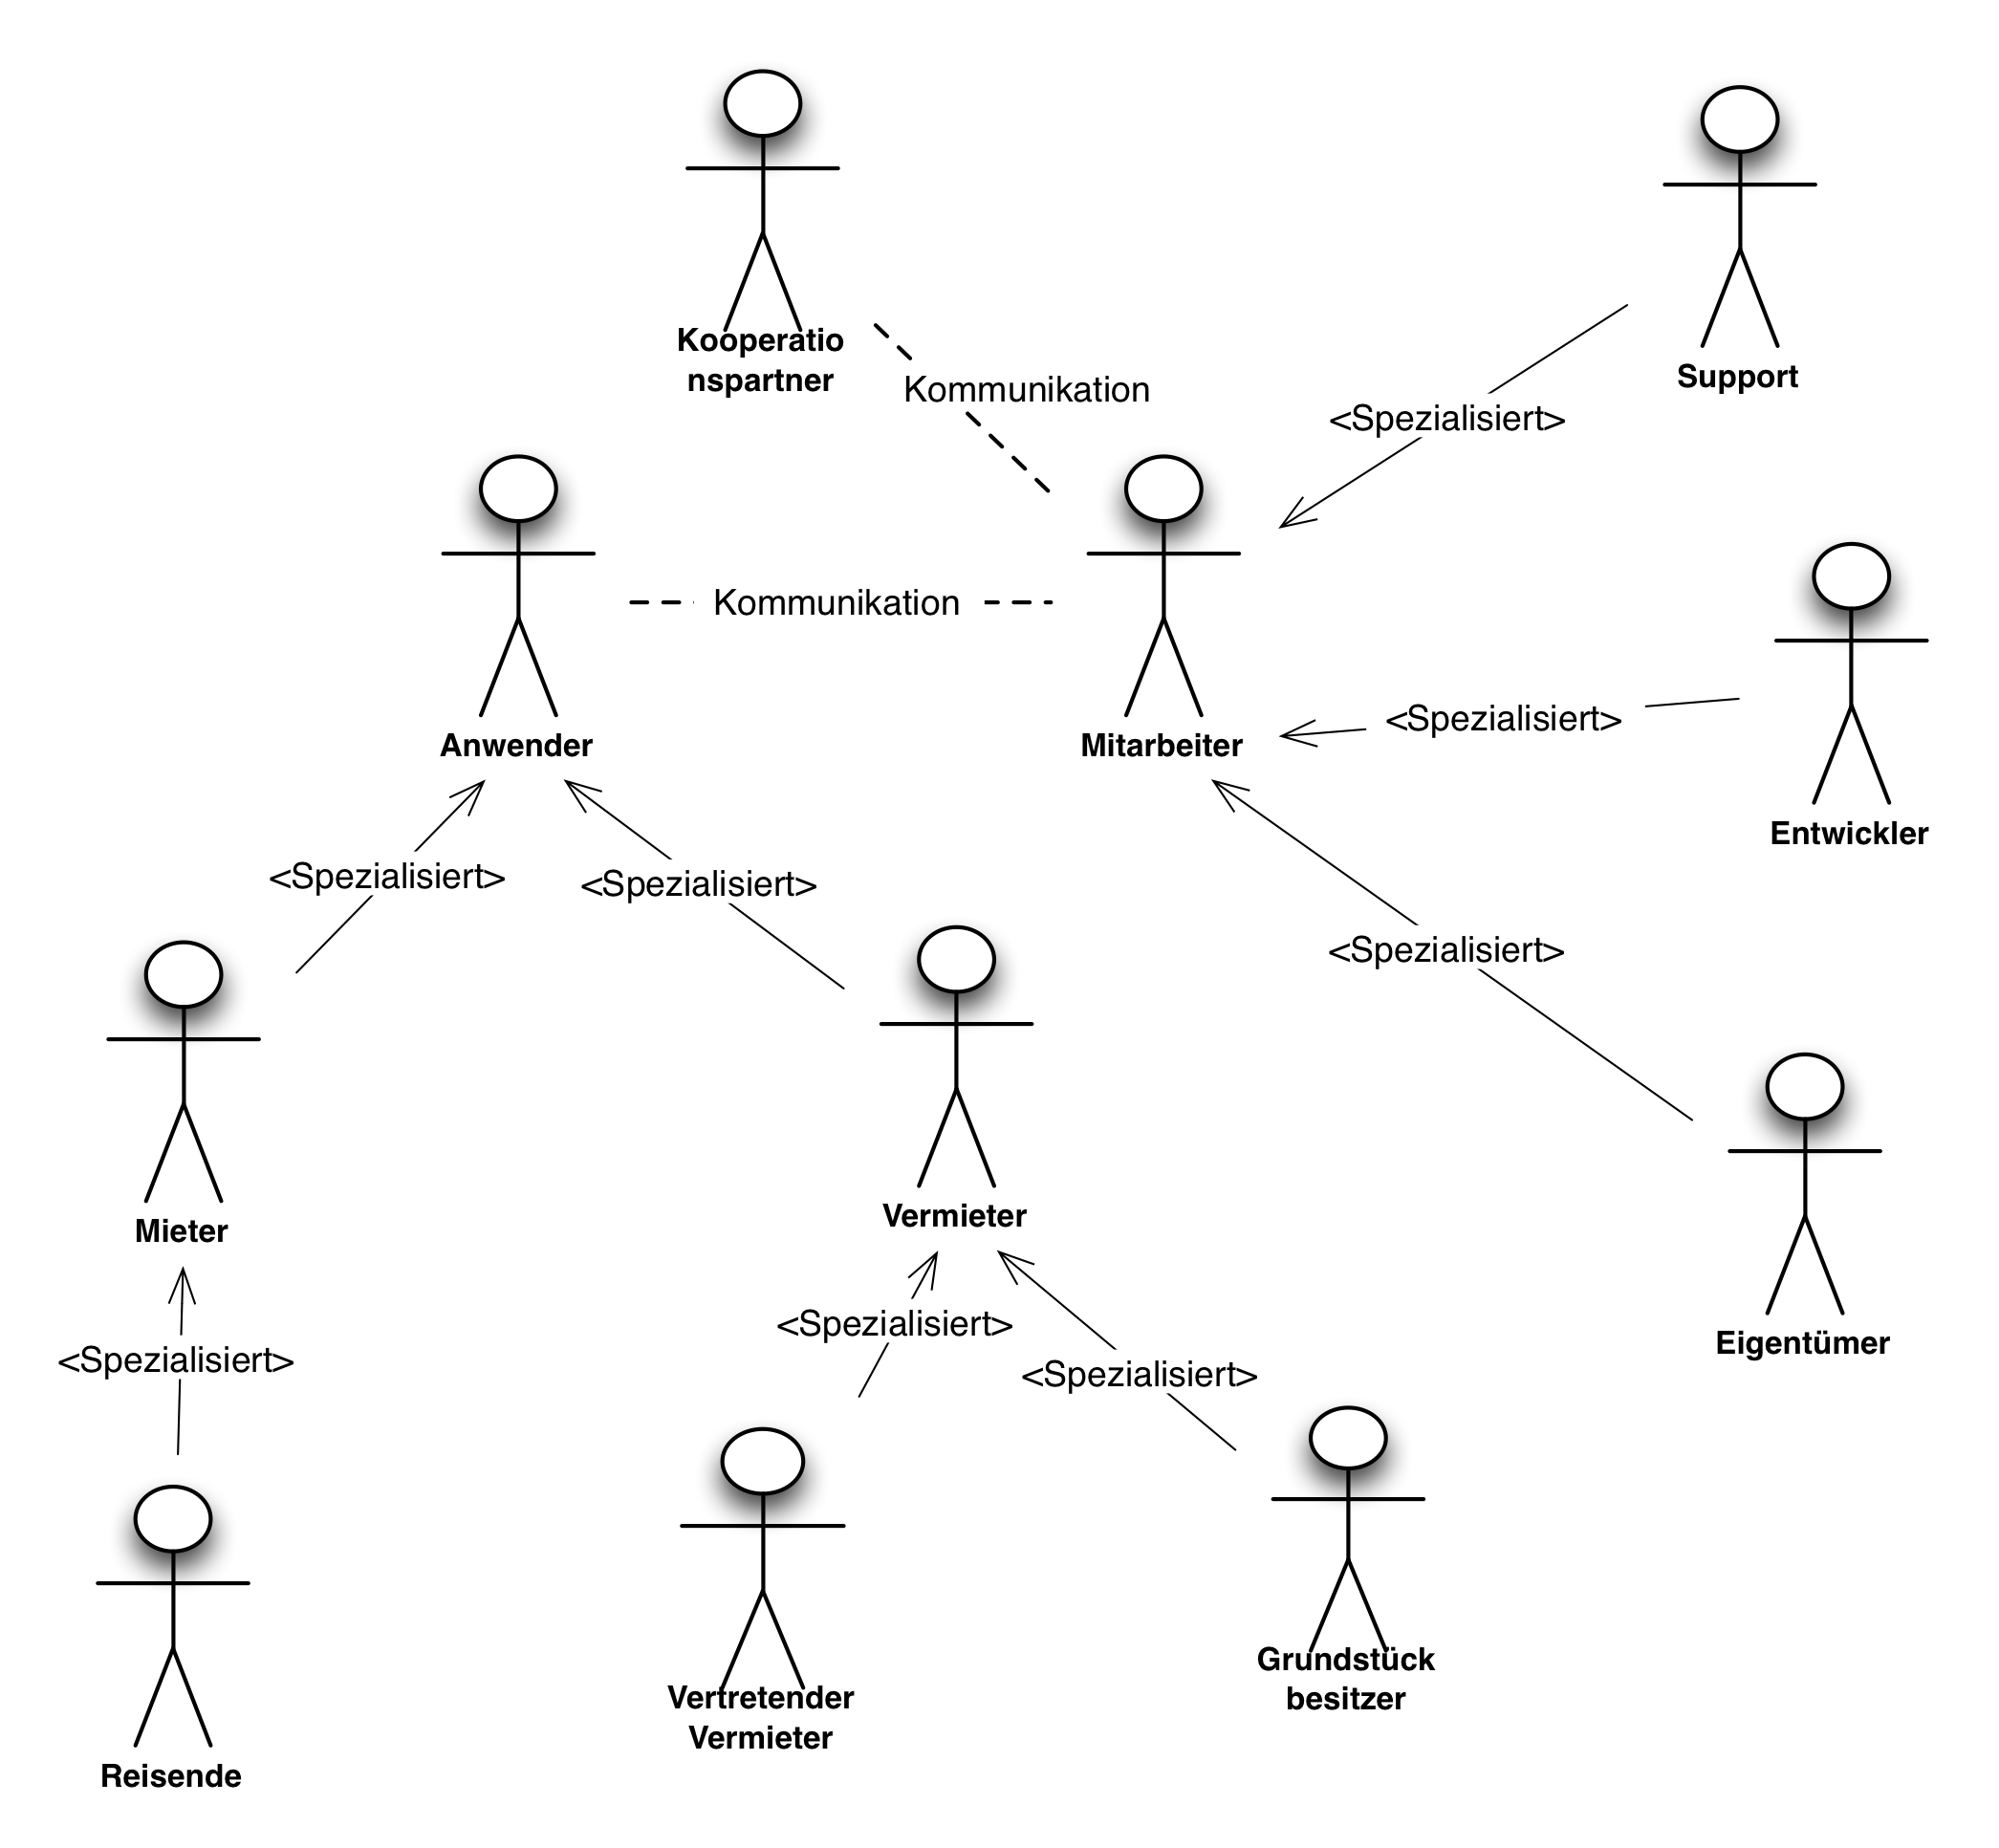
\includegraphics[width=0.75\textwidth]{./images/rolemodeling.png}
\caption{Entwurf der User Role Map}
\label{fig:rolemap}
\end{figure}

Grundsätzlich gibt es 3 Rollentypen, die sich wiederrum in Untertypen Einteilen lassen. Zum einen die Anwender, die als direkte Interessenten mit der Appplikation interagieren. Hierzu zählen die Personen in der Rolle des Mieters und Vermieters. Dabei ist es auch möglich, dass eine Personen zu bestimmten Zeiten eine der Rollen wechselt. Zu den Vermietern zählen die Grundstückbesitzer, die als primary user selber die Vermietung anbieten oder vertretende Vermieter. Damit sind die Personen gemeint, die das Grundstück nicht als Eigentümer besitzen, jedoch von diesem zur Vermietung beauftragt werden.
Eine zweiter Haupttyp ist der Mitarbeiter. In dargestellter Abbildung steht er in direkter Kommunikation mit Anwender, sei es als Supportkraft, Entwickler oder Eigentümer. In dieser Hinsicht ist die Bezeichnung des "Anwenders" eventuell ungünstig gewählt, da auch ein Mitarbeiter bei der Benutzung zum Anwender wird. Diese Trennung spiegelt dabei die Einstufung des internen und externen Stakeholders wieder. Zusätzlich dazu gibt es die Rolle des Kooperationspartners. Er steht in Kommunikation mit Mitarbeiter zur Organisation der Verträge und Absprachen, muss auf Dauer aber nicht zwangsläufig selbst der Benutzer der Applikation sein.




